\chapter{Technology Review}
This chapter discusses the different technologies used in throughout the
project. It discusses the the advantages and disadvantages of each technology 
and why certain technologies were used over others. It also discusses hybrid applications compared to native applications, advantages, disadvantages, uses at different business structures and other topics.

\section{Overview}
This project is a Native android app built with Kotlin in Android Studio, Firebase is used for the database, statistics, verification etc.

Topics:
\begin{itemize}
    \item Kotlin/Java comparison
    \item Fire-base
    \item Picasso
    \item Android Studio/IntelliJ
    \item Native Applications
    \item Hybrid Applications
    \item Hybrid vs Native comparison 
\end{itemize}
\newpage

\section{Main Technologies}
This section will discuss the main technologies currently in use in the android application.

\subsection{Kotlin}
\par
\medskip
\begin{center}
    
\includegraphics[width=12cm,height=12cm,keepaspectratio]{Images/Kotlin.png}
\end{center}
Kotlin is a cross-platform, statically typed, general-purpose programming language with type inference. Kotlin is designed to inter-operate fully with Java, and the JVM version of its standard library depends on the Java Class Library, but type inference allows its syntax to be more concise. Kotlin mainly targets the JVM, but also compiles to JavaScript or native code (via LLVM). Language development costs are borne by JetBrains, while the Kotlin Foundation protects the Kotlin trademark.

Kotlin is the preferred language for Android app developers as of May 2019, since the release of Android Studio 3.0 in October 2017, Kotlin has been included as an alternative to the standard Java compiler. The Android Kotlin compiler targets Java 6 by default, and lets programmers choose between Java 8 to 14 for optimization purposes.

Kotlin originated at JetBrains, which is the company behind IntelliJ IDEA. Kotlin has been open source since 2012 and has a large team of full-time developers working on it, there is also the \hyperlink{https://github.com/JetBrains/kotlin}{Kotlin project of GitHub} which has more than 370 contributors.

\newpage

\subsubsection{Advantages}
Kotlin has many advantages, many are quite serious improvements in readability and workflow which was noticeable when creating my project

\begin{itemize}
    \item \textbf{Less code combined with greater readability} - Spend less time writing code and working to understand the code of others.
    \item \textbf{Mature language and environment} - Kotlin has developed continuously over the years not only as a language but as a whole ecosystem with very robust tooling. Its seamless integration with Android Studio, makes it actively used by companies to develop Android applications.
    \item \textbf{Kotlin support of Android Jetpack and other libraries} - \hyperlink{https://developer.android.com/kotlin/ktx}{KTX extensions} adds kotlin language features, such as coroutines, extension functions, lambdas, and named parameters, to existing Android libraries.
    \item \textbf{Interoperability with Java} - You can use Kotlin along with the Java programming language in your applications without needing to migrate all your code to Kotlin. 
    \item \textbf{Support for multi-platform development} - You can use Kotlin for developing not only Android but also iOS, back-end, and web applications by sharing the common code among the platforms.
    \item \textbf{Code safety} - Less code and better readability lead to fewer errors. The Kotlin compiler detects the remaining errors, making the code safe. 
    \item \textbf{Easy to Learn} - Kotlin is very easy to learn, especially for any Java experienced developers. 
    \item \textbf{Large community} - Kotlin a great support and many contributions from the community, which is growing all over the world. According to Google, over 60\% of the top 100 apps on the Google Play Store use Kotlin. Many startups and Fortune 500 companies have already developed Android applications using Kotlin and more and more companies are prioritizing Kotlin Native application development over other options due to the robust toolkit and optimizations that make your applications the best that they can be. 
\end{itemize}

\newpage

\subsubsection{Disadvantages}

\begin{itemize}
    \item \textbf{Shift from Java to Kotlin} - Kotlin is an amazing programming language and there is a reason why leading lead companies have started using kotlin, but at their core their two different languages. Developers won't be able to quickly shift from one to another without taking time to learn Kotlin. Therefore company's have to consider different approaches to Android app development as additional expenses are required on training a team of developers. 
    \item \textbf{Hard to find experienced developers} - There is a high demand for specialists in Kotlin as Google made it the preferred language for Android development in 2019, but there is still a very large amount of Java programmers on the market compared to Kotlin developers. This means on average the Kotlin developers may be younger meaning less senior developers available for hire. This is quite a large disadvantage, but will quickly fade away as many leading tech companies have switched which creates a ripple effect down the chain of companies.
    \item \textbf{Limited learning resources} - Although the number of Android app developers who use Kotlin instead of Java increase everyday, there is still a limited number of resources in the market compared to Java. Many College courses will teach Java over Kotlin as both are so similar, meaning most Kotlin developers come from a background in Java and learn to code in Kotlin themselves.
\end{itemize}



\subsection{Kotlin vs Java}
\par
\medskip
\begin{center}
    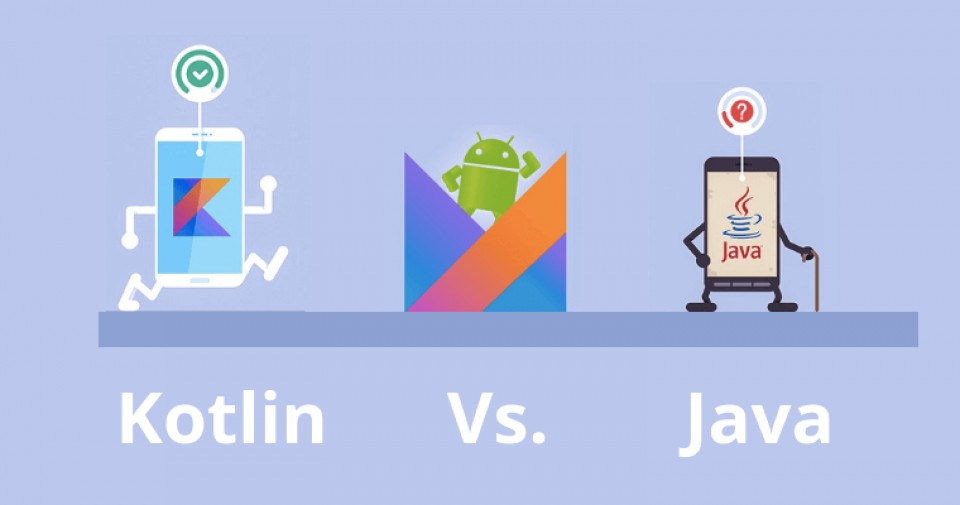
\includegraphics[width=12cm,height=12cm,keepaspectratio]{Images/KotlinvJava.jpg}
\end{center}

\subsection{Firebase}
\par
\medskip
\begin{center}
    
\includegraphics[width=12cm,height=12cm,keepaspectratio]{Images/firebase.png}
\end{center}

\subsection{Picasso}
\par
\medskip
\begin{center}
    
\includegraphics[width=10cm,height=10cm,keepaspectratio]{Images/picasso.png}
\end{center}

\subsection{Native Applications}
\par
\medskip
\begin{center}
    
\includegraphics[width=12cm,height=12cm,keepaspectratio]{Images/nativeapp2.png}
\end{center}

\subsection{Hybrid Applications}
\par
\medskip
\begin{center}
    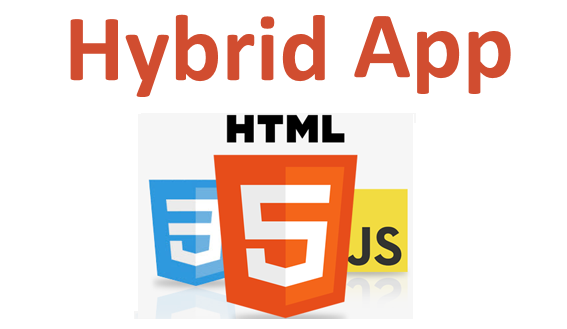
\includegraphics[width=12cm,height=12cm,keepaspectratio]{Images/hybridapp.png}
\end{center}

\subsection{Hybrid vs Native Applications}
\par
\medskip
\begin{center}
    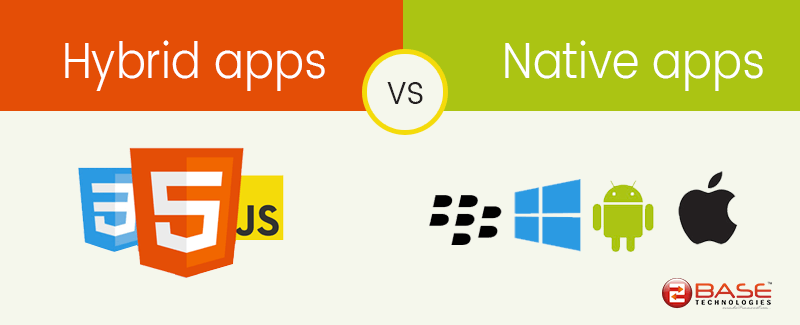
\includegraphics[width=12cm,height=12cm,keepaspectratio]{Images/hybridvnative.png}
\end{center}

\begin{figure}[h!]
	\caption{Hybrid Application}
	\label{image:myImageName}
	\centering
	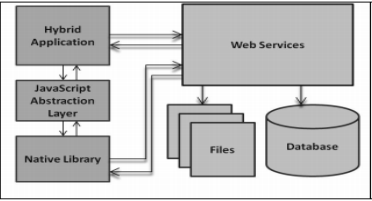
\includegraphics[width=1\textwidth]{Images/hybrid_dev_img.PNG}
\end{figure}